\documentclass[12pt,a4paper]{article}

% ── Language & Encoding ─────────────────────────────────────────────────────
\usepackage[utf8]{inputenc}
\usepackage[T1]{fontenc}
\usepackage[english]{babel}

% ── Layout & Typography ─────────────────────────────────────────────────────
\usepackage[top=2.5cm, bottom=2.5cm, left=3cm, right=2.5cm]{geometry}
\usepackage{parskip}
\usepackage{amsmath}

% ── Code Listing Style ──────────────────────────────────────────────────────
\usepackage{listings}
\usepackage{xcolor}
\newcommand{\inlinecode}[1]{\colorbox{codebg}{\texttt{#1}}}
\definecolor{codebg}{gray}{0.93} 
\lstset{
    language=C,
    basicstyle=\ttfamily\small,          % Font chữ và kích thước
    keywordstyle=\color{blue}\bfseries,  % Màu cho từ khóa (ví dụ: int, return)
    stringstyle=\color{red},             % Màu cho chuỗi (ví dụ: "Hello")
    commentstyle=\color{green!60!black}, % Màu cho chú thích
    numbers=left,                        % Đánh số dòng bên trái
    numberstyle=\tiny\color{gray},       % Kiểu số dòng
    stepnumber=1,
    breaklines=true,                     % Tự động xuống dòng nếu code quá dài
    frame=single,                        % Đóng khung đoạn code
    tabsize=4,                           % Khoảng cách tab
    showstringspaces=false               % Không hiển thị ký tự khoảng trắng trong chuỗi
}
% ... (Keep the rest of your listing definitions here) ...

% ── Graphics & Hyperlinks ───────────────────────────────────────────────────
\usepackage{graphicx}
\usepackage[colorlinks=true, linkcolor=blue, urlcolor=blue]{hyperref}

% ── Bibliography Setup (ADDED HERE) ─────────────────────────────────────────
\usepackage[style=numeric, sorting=none]{biblatex} 
\addbibresource{references.bib}    % Points to your specific .bib file

\title{\textbf{Project Lab of Embedded Systems}}
\author{Group 15}
\date{May 15, 2026}

\begin{document}
\begin{titlepage}
    \centering
    
    % ── University Logo ──
    % Replace 'TU_Chemnitz_Logo_gruen.svg.png' with your logo file name
    
\includegraphics[width=0.7\textwidth]{imgs/TU_Chemnitz_Logo_gruen.svg.png} \\[0cm]
    
    % ── Department & Chair Info ──
    {\large Department of Electrical Engineering and Information Technology} \\[0.2cm]
    {\large Chair of Measurement and Sensor Technology} \\[3cm]
    
    % ── Document Type & Lab Course ──
    {\huge \textbf{Project Documentation}} \\[0.6cm]
    {\Large ,,Project Lab Embedded Systems``} \\[3.5cm]
    
    % ── Metadata Block (Group & Members) ──
    \begin{flushleft}
    \large
    \begin{tabbing}
        \hspace*{3.5cm} \= \kill
        \textbf{Group:} \> 15 \\ [0.3cm]
        \textbf{Members:} \> Gia Khanh Nguyen \\
                          \> Tuan Minh Le \\
                          \> Minh Quang Vu \\
                          \> Khoi Nguyen Nguyen
    \end{tabbing}
    \end{flushleft}
    
    \vspace{1cm}
    
    % ── Project Title ──
    {\large Project: \textbf{Evaluation of Mini-Belt Characterization System using Impedance Spectroscopy}} \\[1cm]
    
    \vfill
    
    % ── Date Block ──
    \begin{flushleft}
    \large
    \begin{tabbing}
        \hspace*{3.5cm} \= \kill
        \textbf{Date:} \> May 15, 2026
    \end{tabbing}
    \end{flushleft}

\end{titlepage}
% \maketitle
\tableofcontents
\newpage

% ── Sub-sections ────────────────────────────────────────────────────────────
\section{Introduction}
% \large \texttt{main.c} -- STM32H7 EIS Signal Processing
% TODO: Write project description.The Mini-Belt Characterization System is an automated, in-line material analysis platform that combines STM32-based Electrochemical Impedance Spectroscopy (EIS) with a miniature conveyor belt and Interdigitated Electrodes (IDEs)[cite: 95]. The system is designed to perform real-time quality monitoring of moving materials, analyzing factors such as moisture content, freshness, and curing state without stopping the production line[cite: 96]. This architecture is specifically targeted for research into smart manufacturing and food processing applications[cite: 98].

% \subsection{Methodology and System Architecture}
% Instead of relying on static lab measurements, the system utilizes Multisine broadband excitation to capture high-speed impedance fingerprints as samples pass over the characterization zone[cite: 97]. To achieve this, the project integrates hardware, software, and machine learning components across several key sub-systems.

% \begin{itemize}
%     \item \textbf{Miniature Conveyor Hardware:} A compact belt assembly is driven by a stepper motor for precise speed control[cite: 101]. It utilizes a "floating header" sensor mount to ensure consistent IDE contact with the moving samples[cite: 102]. Additionally, an optical encoder tracks the belt's position to allow for accurate timestamp correlation[cite: 103, 112].
    
%     \item \textbf{Multisine Signal Generation:} The STM32 Digital-to-Analog Converter (DAC) generates an optimized broadband excitation signal ranging from 1 Hz to 10 kHz[cite: 105]. This output is DMA-driven to ensure jitter-free synthesis, and incorporates phase optimization algorithms to minimize the crest factor[cite: 106, 107].
    
%     \item \textbf{EIS Acquisition and Processing:} High-speed Analog-to-Digital Converters (ADCs) sample the voltage and current with precise phase alignment[cite: 109]. The complex impedance is extracted in real time using on-chip FFT-based Discrete Fourier Transform (DFT) computations.
% \end{itemize}

% \subsection{Data Synchronization, Visualization, and Machine Learning}
% To map the material properties spatially, the system dynamically adjusts its sampling rates based on the conveyor speed and generates impedance versus belt position heatmaps[cite: 113, 114]. The acquired spectral data is streamed via UART or USB-CDC to a host machine[cite: 118]. On the host side, a Python-based graphical user interface (built with matplotlib or pyqtgraph) visualizes the data through real-time Nyquist and Bode plots[cite: 116]. Finally, the system leverages machine learning algorithms to perform real-time characterization of the analyzed materials[cite: 117].
\subsection{Abstract}
The Mini-Belt Characterization System is an automated, in-line material analysis platform designed to perform real-time quality monitoring without stopping the production line. The architecture integrates an STM32-based Electrochemical Impedance Spectroscopy (EIS) module with a miniature conveyor belt and a "floating header" mount for Interdigitated Electrodes (IDEs). \textbf{To capture high-speed impedance fingerprints from moving samples, the system utilizes an optimized Multisine broadband excitation ranging from 1 Hz to 10 kHz, which is DMA-driven for jitter-free synthesis and optimized for crest factor minimization}. An optical encoder tracks the belt's position for precise timestamp correlation, enabling dynamic sampling rate adjustments and the generation of spatial impedance heatmaps. Complex impedance is extracted in real time via on-chip FFT-based Discrete Fourier Transform (DFT) computations. The data is then streamed via UART or USB-CDC to a Python-based host interface for real-time visualization—including Nyquist and Bode plots—and further evaluated using machine learning algorithms. Ultimately, this system is targeted for research into smart manufacturing and food processing applications, providing continuous assessments of parameters such as moisture content, freshness, and curing state.
% \subsection{Project overview}

% This report details the development of the Mini-Belt Characterization System, an automated, small-scale conveyor platform designed for the continuous analysis of materials in motion. The system leverages an STM32 microcontroller and Electrochemical Impedance Spectroscopy (EIS) to facilitate real-time quality monitoring—such as assessing moisture content, curing state, or freshness—without necessitating interruptions to the production line. 

% In contrast to traditional, stationary laboratory measurements, the implemented architecture employs broadband Multisine signals to rapidly acquire the impedance fingerprints of materials as they traverse over Interdigitated Electrodes (IDEs). By integrating custom mechanical hardware, embedded signal processing, and machine learning algorithms, this project presents a viable real-time monitoring solution highly applicable to smart manufacturing and food processing environments.

\subsection{Project outline}
This report is structured to provide a comprehensive overview of the system's development, theoretical foundation, and empirical validation. The subsequent sections are organized as follows:

\begin{itemize}
    \item \textbf{Section 1 (Introduction):} This section will present the research problem and overall objectives of the work. It establishes the context by outlining the relevance of Mini-Belt Characterization System using Impedance Spectroscopy and defining the scope of this project.

    \item \textbf{Section 2 (Theoretical Background):} This section provides the foundational scientific and mathematical principles governing the system. It covers the fundamentals of Electrochemical Impedance Spectroscopy (EIS) and the rationale for utilizing Multisine broadband excitation. Additionally, it details the specific signal processing algorithms—namely, the Fast Fourier Transform (FFT) and the Goertzel algorithm—employed for on-chip impedance calculation, \textbf{alongside an introduction to the machine learning concepts used for material characterization}.
    
    \item \textbf{Section 3 (Hardware and Software Implementation):} This segment details the engineering and architectural design of the platform. It is subdivided into hardware design (encompassing the miniature conveyor, stepper motor, optical encoder, and floating header Interdigitated Electrode mechanism), embedded firmware development (focusing on the STM32 microcontroller configuration and DMA-synchronized data acquisition), and host interface architecture (detailing the Python-based graphical interface and data streaming protocols).
    
    \item \textbf{Section 4 (Experiments and Results):} This section outlines the testing methodology and presents the data gathered during system validation. It includes an evaluation of the multisine signal generation, verifies the accuracy of the EIS measurements through Nyquist and Bode plots, and analyzes the impact of conveyor belt velocity on signal fidelity. Furthermore, it presents the results of the machine learning classification models applied to the material samples.
    
    \item \textbf{Section 5 (Conclusion):} The final section synthesizes the project's outcomes, assessing the overall efficacy of the real-time, in-line characterization system. It critically discusses the technical limitations encountered during the development phase and proposes potential avenues for future enhancement, such as accommodating higher operational speeds or optimizing the sensor topology.
\end{itemize}

\subsection{General objective}
            % Part 1
\section{Theory Background}
\subsection{Electrochemical Impedance Spectroscopy (EIS)}
   % Part 2
\section{Code Understanding}
The \texttt{main.c} file implements an embedded impedance spectroscopy system on an STM32 microcontroller. It generates a multi-sine excitation signal via DAC, acquires the hardware response simultaneously through two independent ADCs using DMA, and processes the signals in the frequency domain using either the Fast Fourier Transform (FFT) or the Goertzel algorithm.

\subsection{Setup}
\begin{lstlisting}
// Start DMA / DAC 3
HAL_DAC_Start_DMA(&hdac1, DAC_CHANNEL_1, signal, SIGNAL_LENGTH, DAC_ALIGN_12B_R);
HAL_TIM_Base_Start(&htim4);

serialPrint(&huart3, "Calibrating ADCs\r\n");
// Calibrate ADCs
HAL_ADCEx_Calibration_Start(&hadc1, ADC_CALIB_OFFSET, ADC_SINGLE_ENDED);
HAL_ADCEx_Calibration_Start(&hadc2, ADC_CALIB_OFFSET, ADC_SINGLE_ENDED);

serialPrint(&huart3, "Starting ADC1/2, TIM2, DMA\r\n");
// Start DMA & ADC 1/2
HAL_ADC_Start_DMA(&hadc1, (uint32_t *)AdcBuffer1, ACQ_LENGTH);
HAL_ADC_Start_DMA(&hadc2, (uint32_t *)AdcBuffer2, ACQ_LENGTH);

HAL_TIM_Base_Start(&htim2);

serialPrint(&huart3, "Forwarding to main loop...\r\n");
\end{lstlisting}

\begin{itemize}

    \item \textbf{Signal Generation (DAC \& TIM4):} The Digital-to-Analog Converter (DAC) is started in DMA mode. This allows the hardware to continuously stream the predefined excitation array ( \inlinecode{signal} ) to the analog output pin without CPU intervention. Timer 4 ( \inlinecode{htim4} ) is enabled to act as the trigger source, dictating the precise update rate of the DAC.

    \item \textbf{Hardware Calibration:} Both Analog-to-Digital Converters (ADC1 and ADC2) undergo an internal self-calibration process. This crucial step compensates for inherent physical offset errors, ensuring high accuracy for subsequent phase and magnitude calculations.

    \item \textbf{Data Acquisition (ADC, TIM2 \& DMA):} The ADCs are activated in DMA mode to continuously capture incoming voltage levels and route the raw data directly into designated memory arrays ( \inlinecode{AdcBuffer1} and \inlinecode{AdcBuffer2} ). Finally, Timer 2 ( \inlinecode{htim2} ) is started to serve as the master sampling clock, establishing a strict sampling frequency for both ADCs.

\end{itemize}
\vspace{1.5cm}
\begin{lstlisting}
if ((DmaCpltFlag1 == 1))
{
    DmaCpltFlag1 = 0;
    HAL_TIM_Base_Stop(&htim2);
    .
    .
    .
    HAL_TIM_Base_Start(&htim2);
}
\end{lstlisting}

\begin{itemize}
    \item \textbf{Condition Check \& Flag Reset:} The system checks if the DMA has completely filled the buffer (\texttt{DmaCpltFlag1 == 1}). If true, the flag is immediately reset to 0 to acknowledge the completion event.

    \item \textbf{Pause Acquisition (\texttt{HAL\_TIM\_Base\_Stop}):} Timer 2, which serves as the trigger source for the ADC, is halted. This safely "freezes" the acquisition process, ensuring the data buffer remains stable and preventing ADC overrun errors.

    \item \textbf{Resume Acquisition (\texttt{HAL\_TIM\_Base\_Start}):} Once the CPU finishes processing the current data block, Timer 2 is reactivated to trigger the ADC again, starting the next data acquisition cycle.
\end{itemize}

\subsection{Signal Processing}
4 modes: \inlinecode{SIGNAL\_OUT}, \inlinecode{SIGNAL\_OUT\_SERIALPLOT\_STYLE}, \inlinecode{FFT}, \inlinecode{GOERTZEL}

\subsubsection{\inlinecode{SIGNAL\_OUT} defined?}
\begin{lstlisting}
#ifdef SIGNAL_OUT
    char message[20];
    int cnt = 0;

    serialPrint(&huart3, "Signal writing...\r\n");
    for (cnt = 0; cnt < ACQ_LENGTH; cnt++)
    {       
#ifdef SIGNAL_OUT_SERIALPLOT_STYLE
        sprintf(message, "%d,%d\r\n", AdcBuffer1[cnt], AdcBuffer2[cnt]);
        HAL_UART_Transmit(&huart3, (uint8_t *)message, strlen(message), 500);

#else
        sprintf(message, "ADC1(%4d)=%4d;\r\n", cnt + 1, AdcBuffer1[cnt]);
        HAL_UART_Transmit(&huart3, (uint8_t *)message, 18, 500);

        sprintf(message, "ADC2(%4d)=%4d;\r\n", cnt + 1, AdcBuffer2[cnt]);
        HAL_UART_Transmit(&huart3, (uint8_t *)message, 18, 500);

#endif

        //

        //	  	  		 	HAL_Delay(10);
    }
    serialPrint(&huart3, "Signal writing done\r\n");
#endif
\end{lstlisting}

\begin{itemize}
    \item \textbf{\inlinecode{SIGNAL\_OUT\_SERIALPLOT\_STYLE} defined}: If this macro is defined, the output format is optimized for real-time plotting tools (e.g., SerialPlot). Each line contains a pair of ADC values separated by a comma, making it easy for plotting software to parse and visualize the data in real time.
    \item \textbf{\inlinecode{SIGNAL\_OUT\_SERIALPLOT\_STYLE} not defined}: The output is more verbose and human-readable. Each ADC value is printed on a separate line with an index, which is useful for debugging or offline analysis but less efficient for real-time plotting.

\end{itemize}

\subsubsection{\inlinecode{FFT} defined?}
\begin{lstlisting}
#ifdef FFT

      uint8_t message[50];

      float32_t Magnitude[SIZE_F];
      float32_t Magnitude1[SIZE_F];
      float32_t Magnitude2[SIZE_F];
      float32_t Phase[SIZE_F];
      float32_t Theta1[SIZE_F];
      float32_t Theta2[SIZE_F];

      float32_t fft_inputbuf[ACQ_LENGTH * 2];
      // int16_t fft_inputbuf[ACQ_LENGTH * 2];
      for (int i = 0; i < ACQ_LENGTH; i++)
      {

        fft_inputbuf[i * 2] = AdcBuffer1[i];
        fft_inputbuf[i * 2 + 1] = 0;
      }

      if(ACQ_LENGTH==2048)       arm_cfft_f32(&arm_cfft_sR_f32_len2048, fft_inputbuf, 0, 1);
      else if(ACQ_LENGTH == 4096) arm_cfft_f32(&arm_cfft_sR_f32_len4096, fft_inputbuf, 0, 1);

  //     if(ACQ_LENGTH==2048)       arm_cfft_q15(&arm_cfft_sR_q15_len2048, fft_inputbuf, 0, 1);
    //     else if(ACQ_LENGTH == 4096) arm_cfft_q15(&arm_cfft_sR_q15_len4096, fft_inputbuf, 0, 1);


      for (int i = 0; i < SIZE_F; i++)
      {

        float32_t in1 = fft_inputbuf[f_freqbins_map[i] * 2];
        float32_t in2 = fft_inputbuf[f_freqbins_map[i] * 2 + 1];
        Theta1[i] = atan2(in2, in1);

        float32_t input1 = fft_inputbuf[f_freqbins_map[i] * 2];
        float32_t input2 = fft_inputbuf[f_freqbins_map[i] * 2 + 1];
        Magnitude1[i] = (float)sqrt((input1 * input1) + (input2 * input2));

      } // FFT_ADC1_END

      // FFT_ADC2_ START
      for (int i = 0; i < ACQ_LENGTH; i++)
      {

        fft_inputbuf[i * 2] = AdcBuffer2[i];
        fft_inputbuf[i * 2 + 1] = 0;
      }

      if(ACQ_LENGTH==2048) arm_cfft_f32(&arm_cfft_sR_f32_len2048, fft_inputbuf, 0, 1);
      else if(ACQ_LENGTH == 4096) arm_cfft_f32(&arm_cfft_sR_f32_len4096, fft_inputbuf, 0, 1);

      //     if(ACQ_LENGTH==2048)       arm_cfft_q15(&arm_cfft_sR_q15_len2048, fft_inputbuf, 0, 1);
        //     else if(ACQ_LENGTH == 4096) arm_cfft_q15(&arm_cfft_sR_q15_len4096, fft_inputbuf, 0, 1);

      for (int i = 0; i < SIZE_F; i++)
      {

        float32_t in1 = fft_inputbuf[f_freqbins_map[i] * 2];
        float32_t in2 = fft_inputbuf[f_freqbins_map[i] * 2 + 1];
        Theta2[i] = atan2(in2, in1);

        float32_t input1 = fft_inputbuf[f_freqbins_map[i] * 2];
        float32_t input2 = fft_inputbuf[f_freqbins_map[i] * 2 + 1];

        Magnitude2[i] = (float)sqrt((input1 * input1) + (input2 * input2));

        Phase[i] = (float)((Theta1[i] - Theta2[i]) * (180 / PI)) + 180; //+90;
        Phase[i] = fmod(Phase[i] - 360, 360);
        Magnitude[i] = (float)(Magnitude1[i] / Magnitude2[i]) * 1000;

        //accumulate
        if (accPhase[i] == 0) accPhase[i] = Phase[i];
        if (accMagnitude[i] == 0) accMagnitude[i] = Magnitude[i];
        accPhase[i] = accPhase[i] * accFactor + Phase[i] * (1-accFactor);
        accMagnitude[i] = accMagnitude[i] * accFactor + Magnitude[i] * (1-accFactor);
      }
\end{lstlisting}

\begin{itemize}
    \item \textbf{Data Formatting for CMSIS-DSP (\texttt{fft\_inputbuf}):} The \texttt{arm\_cfft\_f32} function requires a complex input array where real and imaginary parts are interleaved. The loop fills the even indices with raw ADC data (Real part) and sets the odd indices to 0 (Imaginary part).
    
    \item \textbf{Fast Fourier Transform Execution:} The hardware-accelerated 32-bit floating-point FFT function (\texttt{arm\_cfft\_f32}) is executed. It dynamically selects the pre-computed twiddle factor tables (\texttt{arm\_cfft\_sR\_f32\_len2048} or \texttt{4096}) based on the defined acquisition length (\texttt{ACQ\_LENGTH}). Fixed-point operations (\texttt{q15}) are commented out, indicating a preference for floating-point precision over execution speed in this phase.
    
    \item \textbf{Magnitude \& Phase Extraction:} Rather than processing the entire spectrum, the algorithm optimally extracts data only at specific target frequency bins defined by \texttt{f\_freqbins\_map}. For both ADC1 and ADC2:
    \begin{itemize}
        \item Phase (\texttt{Theta}) is calculated using the four-quadrant inverse tangent function (\texttt{atan2(imaginary, real)}).
        \item Magnitude is computed using the Euclidean distance: $\sqrt{\mathrm{real}^2 + \mathrm{imaginary}^2}$.
    \end{itemize}
    
    \item \textbf{Relative Signal Analysis:} The core objective of the system is evaluated here:
    \begin{itemize}
        \item \textbf{Relative Phase:} The phase difference between ADC1 and ADC2 is calculated, converted from radians to degrees (\texttt{180 / PI}), shifted by an offset, and then wrapped within a 360-degree range using the modulo function (\texttt{fmod}).
        \item \textbf{Relative Magnitude:} The magnitude ratio (\texttt{Magnitude1 / Magnitude2}) is calculated and scaled by a factor of 1000.
    \end{itemize}
    
    \item \textbf{Data Smoothing (Exponential Moving Average):} To mitigate high-frequency noise and stabilize the readings over multiple acquisition cycles, an IIR (Infinite Impulse Response) filter is applied to the final values. The accumulated values (\texttt{accPhase} and \texttt{accMagnitude}) are updated using a weighting factor (\texttt{accFactor}), prioritizing historical data while slowly incorporating new measurements.
\end{itemize}  % Part 3
\section{Hardware Setup}
\subsection{Circuit Design}
% The evaluation circuit is primarily composed of three AD8421 instrumentation amplifiers \cite{ad8421_datasheet} and one ADA4522 operational amplifier \cite{ada4522_datasheet}. To facilitate a systematic analysis, the circuit can be divided into distinct functional partitions.

% \subsection{System Architecture Overview}

The hardware front-end for the impedance spectroscopy measurement system is designed to generate a precisely conditioned excitation signal, apply it to the target load, and capture the resulting differential voltage and current. To facilitate a clear understanding of the signal flow, the circuit is logically partitioned into five sequential stages, which is also depicted here in \ref{fig:overal-circuit}:

\begin{figure}[h!]
    \centering
    
\includegraphics[width=1\textwidth]{New_circuit.png}
    \caption{Overal circuit in LTSpice}
    \footnotemark
    \label{fig:overal-circuit}
\end{figure}


\begin{enumerate}
    \item \textbf{Stage 1: DC Reference Generation:} The system begins by establishing a highly stable 1.65V DC reference voltage. This bias is derived from the main 5V supply and buffered to provide a low-impedance foundation. This ensures that the single-supply Analog-to-Digital Converters (ADCs) and instrumentation amplifiers can operate around a centered, virtual ground.
    
    \item \textbf{Stage 2: Signal Conditioning (DAC Output):} A unipolar multisine excitation signal (ranging from 0.0V to 3.3V) is generated by the STM32 microcontroller. This stage utilizes an instrumentation amplifier to subtract the 1.65V reference from the source, effectively level-shifting the waveform into a bipolar AC signal (-1.65V to +1.65V). This critical step prevents DC polarization of the target load.
    
    \item \textbf{Stage 3: The Device Under Test (DUT):} The conditioned AC signal is driven into the measurement path. This physical path consists of the target impedance network (the DUT) connected in series with a known precision shunt resistor to ground. 
    
    \item \textbf{Stage 4: Differential Voltage Measurement ($U_v$):} A dedicated instrumentation amplifier is positioned directly across the DUT to measure the precise voltage drop. This differential AC signal is captured and level-shifted back to a 1.65V DC center to match the unipolar input requirements of the microcontroller's ADC.
    
    \item \textbf{Stage 5: Current Measurement ($U_i$):} A parallel instrumentation amplifier measures the voltage drop across the series shunt resistor. Because the shunt resistance is a known constant, this voltage is directly proportional to the current flowing through the DUT. Like the voltage measurement, this signal is level-shifted and filtered before being routed to the ADC.
\end{enumerate}

By capturing both the $U_v$ and $U_i$ signals simultaneously through these five stages, the microcontroller can perform discrete Fourier transforms // Goertez algorithm on the synchronized data to calculate the complex impedance of the DUT across the generated frequency spectrum.

\subsubsection{Stable 1.65V Reference Supply}\label{sec:1.65}
% A stable 1.65\,V reference voltage is required to bias the Digital-to-Analog Converter (DAC) and Analog-to-Digital Converter (ADC) components without introducing drift. This is achieved using a voltage divider network connected to a stable 5\,V source. The divider consists of a 6.7\,k$\Omega$ and a 3.3\,k$\Omega$ resistor, scaling the voltage appropriately:

% \begin{equation}
%     V_{ref} = 5\,\text{V} \times \frac{3.3\,\text{k}\Omega}{6.7\,\text{k}\Omega + 3.3\,\text{k}\Omega} = 1.65\,\text{V}
% \end{equation}

% The scaled voltage is subsequently filtered through a 10\,$\mu$F capacitor to attenuate high-frequency noise. Finally, the signal is buffered using an ADA4522 operational amplifier configured as a voltage follower. This configuration provides a low-impedance output for the 1.65\,V reference, ensuring stability under varying load conditions from the downstream components \cite{ada4522_datasheet}.

A stable reference voltage (nominally 1.65\,V) is required to bias the Digital-to-Analog Converter (DAC) and Analog-to-Digital Converter (ADC) components without introducing drift. This is achieved using a voltage divider network connected to a stable 5\,V source. To improve power supply rejection and ensure stability, the 5\,V source is initially decoupled with a $1\,\mu\mathrm{F}$ capacitor (C3).

The voltage divider itself consists of a $680\,\Omega$ resistor ($R_8$) and a $330\,\Omega$ resistor ($R_9$), which scales the voltage according to the standard voltage divider formula:
\begin{equation}
    V_{ref} = 5\,\mathrm{V} \times \frac{330\,\Omega}{680\,\Omega + 330\,\Omega} \approx 1.634\,\mathrm{V}
\end{equation}

This scaled voltage, which provides an effective nominal center point for the $3.3\,\mathrm{V}$ ADC logic, is subsequently filtered through a $10\,\mu\mathrm{F}$ capacitor (C2) to attenuate high-frequency noise. Finally, the signal is buffered using an ADA4522-1 operational amplifier (U6) configured as a voltage follower. This configuration provides a low-impedance output for the reference voltage, ensuring stability under varying load conditions from the downstream components \cite{ada4522_datasheet}.

\subsubsection{The DAC Output Stage}

The DAC partition utilizes an AD8421 instrumentation amplifier (U4) to condition the multisine signal generated by the STM32 microcontroller. The AD8421 is selected for its high common-mode rejection and differential input configuration \cite{ad8421_datasheet}. 

The STM32 generates a unipolar multisine signal ($V_{dac}$) ranging from 0.0\,V to 3.3\,V. To prevent DC polarization in the subsequent ADC stage and the Device Under Test (DUT), this signal must be centered around zero. The AD8421 achieves this by subtracting the buffered reference voltage, mentioned in \textbf{Sec.}\ref{sec:1.65}, from the source signal. 

To appropriately scale the output, this stage utilizes a gain resistor ($R_7$) of $100\,\mathrm{k}\Omega$ connected across the RG pins. According to the AD8421 datasheet \cite{ad8421_datasheet}, the gain $G$ is determined by the equation $G = 1 + \frac{9.9\,\mathrm{k}\Omega}{R_G}$, resulting in a nominal gain of approximately $1.099$.

The general transfer function for the AD8421 is explicitly defined in its datasheet as \cite{ad8421_datasheet}:
\begin{equation}
    V_{OUT} = G \times (V_{+IN} - V_{-IN}) + V_{REF}
\end{equation}

In this circuit configuration, the multisine signal is fed into the non-inverting input ($V_{+IN} = V_{dac}$), the stable reference voltage is connected to the inverting input ($V_{-IN} \approx 1.634\,\mathrm{V}$), and the output reference pin is tied directly to ground ($V_{REF} = 0\,\mathrm{V}$). Substituting these parameters yields the specific output equation:
\begin{equation}
    V_{OUT} = 1.099 \times (V_{dac} - 1.634\,\mathrm{V})
\end{equation}

This mathematical shift effectively translates and slightly amplifies the original unipolar signal into a bipolar AC waveform. 

The physical pin configuration of the AD8421 in this setup is illustrated in Figure \ref{fig:ad8421_pinout} and detailed as follows:
\begin{itemize}
    \item \textbf{Pin 1 (-IN):} Connected to the stable reference supply from U6.
    \item \textbf{Pins 2 \& 3 (RG):} Connected to the $100\,\mathrm{k}\Omega$ gain resistor ($R_7$).
    \item \textbf{Pin 4 (+IN):} Connected to the multisine signal input from the STM32.
    \item \textbf{Pin 5 (-VS):} Connected to the $-5$\,V power supply.
    \item \textbf{Pin 6 (REF):} Connected to system ground (GND).
    \item \textbf{Pin 7 (VOUT):} The conditioned output signal, passed to the DUT.
    \item \textbf{Pin 8 (+VS):} Connected to the $+5$\,V power supply.
\end{itemize}

\begin{figure}[h!]
    \centering
    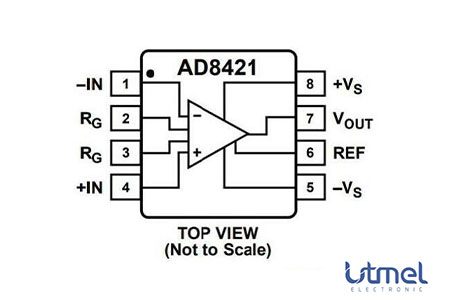
\includegraphics[width=0.6\textwidth]{AD8421.jpg}
    \caption{Pin layout and configuration of the AD8421}
    \footnotemark
    \label{fig:ad8421_pinout}
\end{figure}
\footnotetext{Source: \url{https://www.utmel.com/components/ad8421-amplifier-pinout-datasheet-schematic?id=745}}

% ##############################################################

% The DAC partition utilizes an AD8421 instrumentation amplifier to condition the multisine signal generated by the STM32 microcontroller. The AD8421 is selected for its high common-mode rejection and differential output configuration \cite{ad8421_datasheet}. 

% The AD8421 achieves this by subtracting the 1.65\,V reference from the source signal. The general transfer function for the AD8421 is given by the following equation:
% \begin{equation}
%     V_{OUT} = G \times (V_{+IN} - V_{-IN}) + V_{REF}
% \end{equation}

% By leaving the gain-setting pins (RG) unconnected, the amplifier gain $G$ is set to unity ($G = 1$). The circuit is configured such that the multisine signal is fed into the non-inverting input ($V_{+IN} = V_{dac}$), the stable reference voltage is connected to the inverting input ($V_{-IN} = 1.65\,\text{V}$), and the output reference pin is tied to ground ($V_{REF} = 0\,\text{V}$). Substituting these parameters into the transfer function yields:
% \begin{equation}
%     V_{OUT} = 1 \times (V_{dac} - 1.65\,\text{V}) + 0\,\text{V} = V_{dac} - 1.65\,\text{V}
% \end{equation}

% This mathematical shift effectively translates the original $0.0$\,V to $3.3$\,V unipolar signal into a bipolar signal with an output range of $-1.65$\,V to $+1.65$\,V.

% The STM32 generates a unipolar multisine signal ranging from 0.0\,V to 3.3\,V. To prevent polarization in the subsequent ADC stage and the Device Under Test (DUT), this signal must be centered around zero. The AD8421 achieves this by subtracting the 1.65\,V reference from the source signal. Specifically, the multisine signal is fed into the non-inverting input (IN+), while the stable 1.65\,V reference is connected to the inverting input (IN-). This effectively shifts the output signal range to $-1.65$\,V to $+1.65$\,V.

% The physical pin configuration of the AD8421 in this setup is illustrated in Figure \ref{fig:ad8421_pinout} and detailed as follows:
% \begin{itemize}
%     \item \textbf{Pin 1 (-IN):} Connected to the stable 1.65\,V reference supply.
%     \item \textbf{Pins 2 \& 3 (RG):} Left unconnected to set the amplifier gain to unity ($G = 1$).
%     \item \textbf{Pin 4 (+IN):} Connected to the multisine signal input from the STM32.
%     \item \textbf{Pin 5 (-VS):} Connected to the $-5$\,V power supply.
%     \item \textbf{Pin 6 (REF):} Connected to system ground (GND).
%     \item \textbf{Pin 7 (VOUT):} The conditioned output signal, passed to the DUT.
%     \item \textbf{Pin 8 (+VS):} Connected to the $+5$\,V power supply.
% \end{itemize}

% \begin{figure}[h!]
%     \centering
%     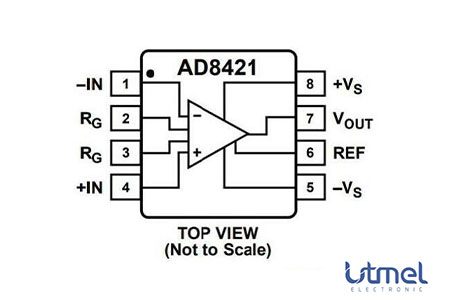
\includegraphics[width=0.6\textwidth]{AD8421.jpg}
%     \caption{Pin layout and configuration of the AD8421}
%     \footnotemark
%     \label{fig:ad8421_pinout}
% \end{figure}
% \footnotetext{Source: \url{https://www.utmel.com/components/ad8421-amplifier-pinout-datasheet-schematic?id=745}}


% The resulting level-shifted multisine waveform from the DAC stage is depicted in Figure \ref{fig:dac_output}. The oscilloscope captures two distinct traces: the prominent yellow trace represents the original multisine input signal generated by the STM32, while the fainter pink trace beneath it displays the conditioned output from the AD8421. 

% As observed in the figure, the output waveform successfully tracks the input with minimal visible noise. However, to further guarantee system stability and limit the effective bandwidth, the AD8421 datasheet suggests introducing a small capacitor into the configuration. Specifically, a $12\,\mathrm{pF}$ capacitor is recommended as a practical starting point to mitigate potential high-frequency instability under varying load conditions \cite{ad8421_datasheet}.

% \begin{figure}[h!]
%     \centering
%     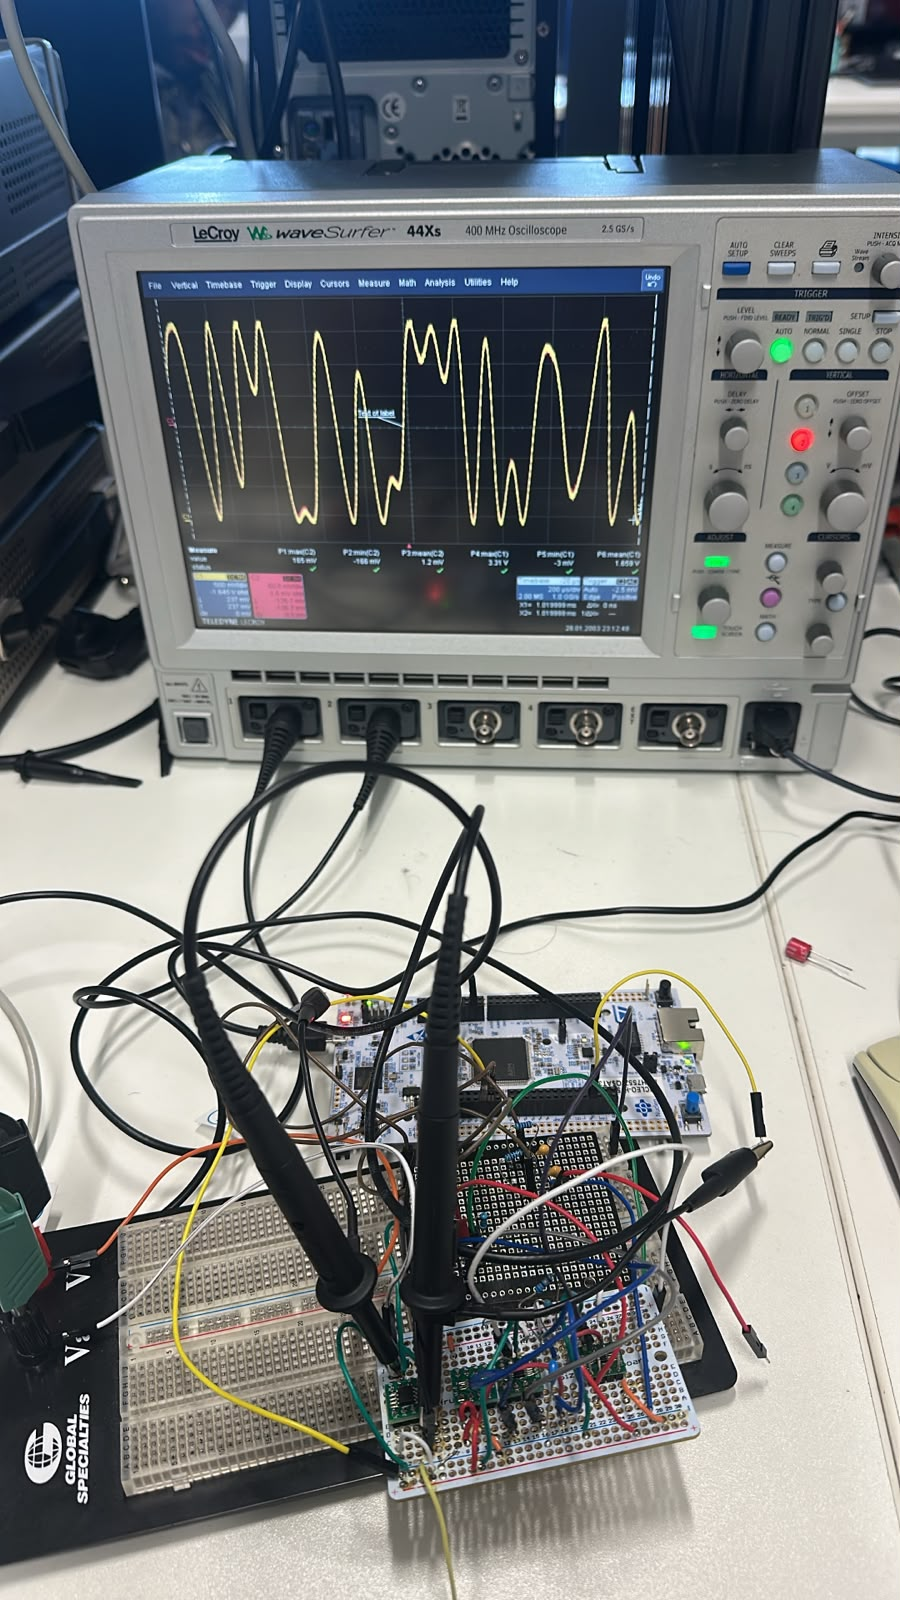
\includegraphics[width=0.5\textwidth]{dac_output.jpeg}
%     \caption{Output waveform of the DAC stage after level shifting via the AD8421.}
%     \label{fig:dac_output}
% \end{figure}
% ##############################################################
% \subsubsection{The DUT}
% The first Device under Test is a 1.5kOhm resistor connected in series with a parallel 4.7nF capacitor and a 1.5kOhm resistor. Another shunt resistor is then connected with the DUT in order to measure the current of the DUT. The output signal of the DAC is then passed to the DUT and the voltage and current are then measured and pass through the ADC component for further analysis.

\subsubsection{The Device Under Test (DUT)}
% To evaluate the measurement system, a known passive component network is utilized as the first Device Under Test (DUT). This network is modeled to represent a typical impedance load and consists of a $1.5\,\mathrm{k}\Omega$ resistor connected in series with a parallel combination of a $47\,\mathrm{nF}$ capacitor and a second $1.5\,\mathrm{k}\Omega$ resistor. 

% To enable current measurement, a $1.5\,\mathrm{k}\Omega$ shunt resistor ($R_{shunt}$) is connected in series with the DUT and tied to ground. When the conditioned multisine signal from the DAC stage is applied to the DUT, the resulting voltage across the DUT and the current flowing through the shunt resistor can be simultaneously captured for impedance spectroscopy analysis.

\subsubsection{The ADC Front-End (Signal Measurement)}
To accurately capture the voltage and current for the microcontroller's Analog-to-Digital Converter (ADC), the measurement stage employs two AD8421 instrumentation amplifiers. These amplifiers provide the necessary high common-mode rejection, low noise, and precise differential sensing required for reliable impedance calculations \cite{ad8421_datasheet}.

\begin{itemize}
    \item \textbf{Voltage Measurement ($U_v$):} The first AD8421 (U1) is configured to measure the differential voltage directly across the DUT. The non-inverting input (+IN) is connected to the node between the DUT and the shunt resistor, while the inverting input (-IN) is connected to the node preceding the DUT. 
    \item \textbf{Current Measurement ($U_i$):} The second AD8421 (U2) is dedicated to current measurement by capturing the voltage drop across the $1.5\,\mathrm{k}\Omega$ shunt resistor. Its non-inverting input (+IN) is tied directly to system ground (GND), and its inverting input (-IN) is connected to the node between the DUT and the shunt resistor.
\end{itemize}

Both amplifiers utilize a gain resistor ($R_G$) of $100\,\mathrm{k}\Omega$. According to the AD8421 transfer function ($G = 1 + 9.9\,\mathrm{k}\Omega / R_G$), this results in a nominal gain of approximately $1.099$. 

Furthermore, to ensure the measured bipolar signals are compatible with the unipolar $0.0\,\mathrm{V}$ to $3.3\,\mathrm{V}$ input range of the STM32's ADC, the reference pins (REF) of both AD8421 amplifiers are tied to the stable $1.65\,\mathrm{V}$ supply described in the previous section. This effectively level-shifts the $U_v$ and $U_i$ AC outputs to a $1.65\,\mathrm{V}$ DC center point.

Finally, in accordance with the manufacturer's recommendations for driving ADCs, the high-bandwidth outputs of the AD8421s should be routed through an RC low-pass filter before reaching the ADC pins. As noted in the component specifications, this filtering isolates the amplifier from the dynamic capacitive loading of the ADC inputs, reduces the effective noise bandwidth, and provides overload protection \cite{ad8421_datasheet}.

% \subsubsection{The ADC Stage}
% % Add your ADC documentation here
% The ADC consisits of 2 INA (AD8421) 

\subsection{Microcontroller and Digital Signal Processing}
The central processing and control unit of the measurement system is the STM32H755ZI-Q microcontroller, housed on a Nucleo-144 development board \cite{stm32_nucleo}.

To ensure strict timing deterministic behavior—which is critical for accurate phase measurements in impedance spectroscopy—the firmware heavily leverages hardware timers and Direct Memory Access (DMA). The code flow correlates directly to the hardware partitions as follows:

\begin{itemize}
    \item \textbf{Signal Generation (DAC \& DMA):} A 4096-point multisine waveform is pre-calculated and stored in the microcontroller's memory. Timer 4 (TIM4) is configured to trigger the Digital-to-Analog Converter (DAC1), while a DMA channel continuously streams the waveform array to the DAC register. This allows the STM32 to output the unipolar excitation signal to the hardware subtractor stage continuously without utilizing CPU cycles. In \textbf{Fig.}\ref{fig:DAC_output}, the multisine wave is measured using the oscilloscope
    
    
    \item \textbf{Simultaneous Acquisition (ADCs \& DMA):} The differential voltage ($U_v$) and current ($U_i$) signals conditioned by the AD8421 front-end are routed to two separate Analog-to-Digital Converters (ADC1 and ADC2). Timer 2 (TIM2) synchronizes both ADCs to sample at the exact same frequency. Two dedicated DMA streams capture 4096 samples into parallel memory buffers (\inlinecode{AdcBuffer1} and \inlinecode{AdcBuffer2}).
    
    \item \textbf{Interrupt and DSP Execution:} Once the DMA completes filling the 4096-point buffers, a hardware interrupt (\inlinecode{HAL\_ADC\_ConvCpltCallback}) sets a completion flag. The main loop halts the acquisition timer and begins processing the buffers. Using the CMSIS-DSP library, the firmware applies the Goertzel algorithm (or alternatively, a Fast Fourier Transform) to the sampled data. This extracts the precise magnitude and phase shift for the specific frequency bins present in the multisine signal.
    
    \item \textbf{Data Transmission:} After calculating the accumulated phase and magnitude, the results are formatted and transmitted via USART3 to a connected PC for final logging and visualization. 
\end{itemize}

\begin{figure}[h!]
        \centering
        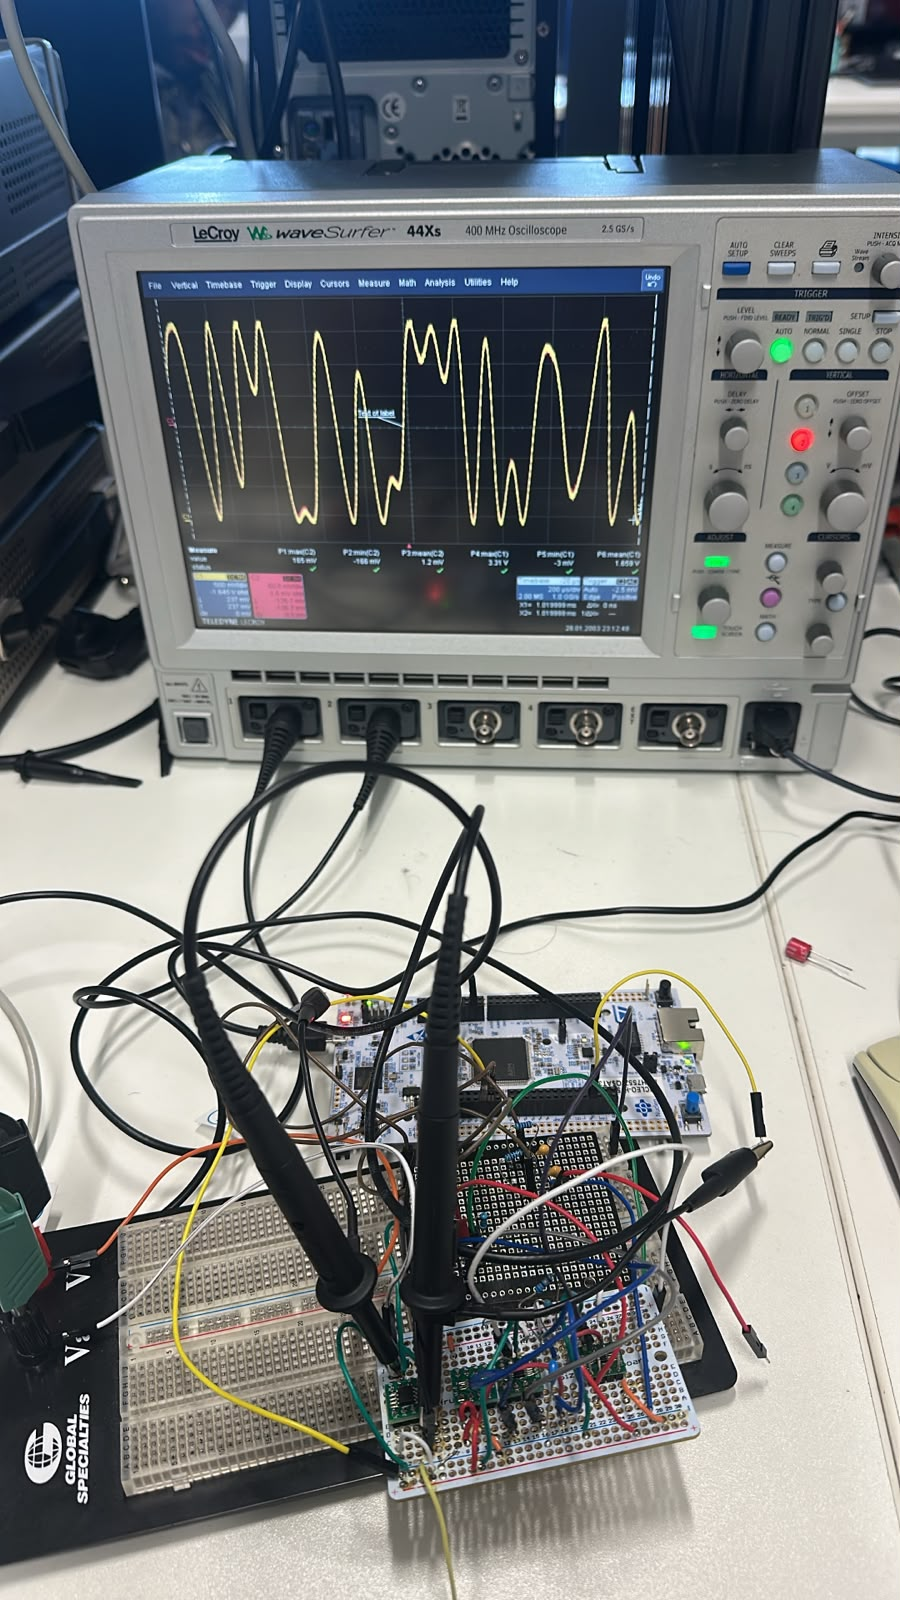
\includegraphics[width=1\textwidth]{dac_output.jpeg}
        \caption{DAC output from STM32 measured by oscilloscope}
        \footnotemark
        \label{fig:DAC_output}
    \end{figure}

\subsubsection{Firmware Execution Flow}
The sequential logic of the firmware, from peripheral initialization to the continuous DSP loop, is illustrated in Figure \ref{fig:stm32_flow_chart}.

\begin{figure}[h!]
    \centering
    
\includegraphics[width=0.8\textwidth]{Diagram_project.png}
    \label{fig:stm32_flow_chart}
    \caption{STM32 execution flow chart}
\end{figure}

\subsection{Setup}      % Part 4


% ── Generate Bibliography Here ──

\end{document}